\documentclass{beamer}
\usepackage{graphicx}
\begin{document}

\title {Anisotropic Math}

\author {Anton Kodochygov}

\begin{frame}
\titlepage
\end{frame}

\begin{frame}
\frametitle{Preliminaries}
\begin{itemize}

\pause \item Eikonal equation (isotropic):
\begin{eqnarray}
|\nabla T| = |p| = U \nonumber
\end{eqnarray}

\pause \item Eikonal equation (anisotropic):
\begin{eqnarray}
|\nabla T| = |p| = U(\xi) \nonumber
\end{eqnarray}

\pause \item Snell's Law (isotropic):
\begin{eqnarray}
sin(\theta_1)/v_1 = sin(\theta_2)/v_2 \nonumber
\end{eqnarray}

\pause \item Snell's Law (anisotropic):
\begin{eqnarray}
sin(\theta_1)/v_1(\xi_1) = sin(\theta_2)/v_2(\xi_2) \nonumber
\end{eqnarray}

\end{itemize}
\end{frame}

\begin{frame}
\frametitle{Snell's Law Intuition}
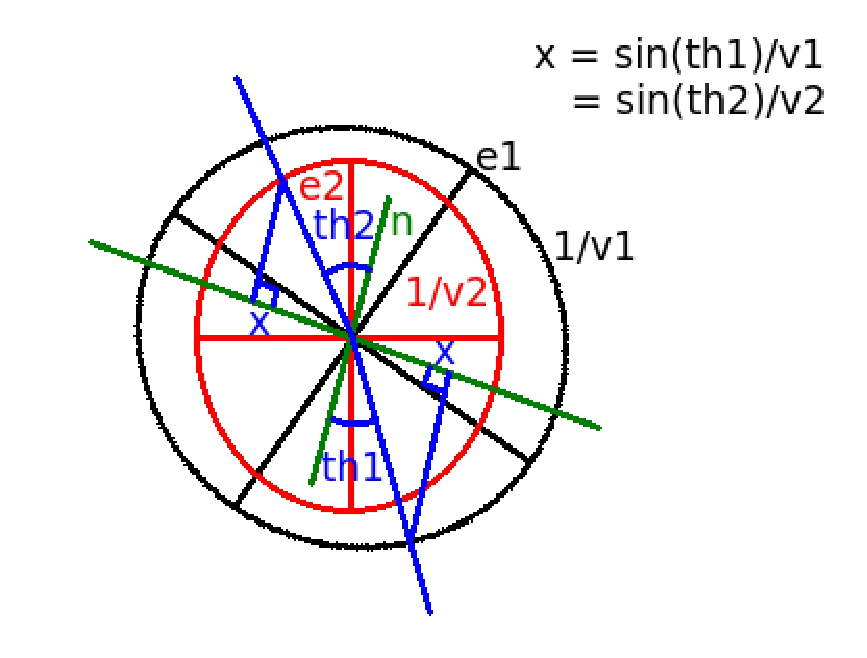
\includegraphics[width=\textwidth]{snell_intuition.eps}
\end{frame}

\begin{frame}
\frametitle{Christoffel Matrix}

\begin{itemize}

\pause \item
Newton's Second Law:

\begin{eqnarray}
\rho \frac{\partial^2 u_i}{\partial t^2} &=& c_{ijkl} \frac{\partial^2 u_i}{\partial x_j \partial x_l} \nonumber
\end{eqnarray}

\pause \item
Christoffel Matrix:

\begin{eqnarray}
G_{ik} &=& c_{ijkl} n_l n_j \nonumber
\end{eqnarray}

\pause \item
Phase Velocities (eigenvectors of G):

\begin{eqnarray}
(G_{ik}-\rho v^2 \delta_{ik} ) \bar{U_k} &=& 0 \nonumber
\end{eqnarray}

\end{itemize}

\end{frame}

\begin{frame}
\frametitle{Stress Tensor Simplification}

\fontsize{6pt}{7.2}\selectfont

\begin{itemize}

\pause \item
The 81 element tensor can be represented by a 6x6 matrix
\begin{eqnarray}
c_{ijkl} &\rightarrow& C_{IJ} \nonumber \\
11 &\rightarrow& 1 \nonumber \\
22 &\rightarrow& 2 \nonumber \\
33 &\rightarrow& 3 \nonumber \\
23 &\rightarrow& 4 \nonumber \\
13 &\rightarrow& 5 \nonumber \\
12 &\rightarrow& 6 \nonumber
\end{eqnarray}

\pause \item
Furthermore, due to symmetry, we can further simplify this matrix

\[ C =  \left( \begin{array}{cccccc}
C_{11} & C_{12} & C_{13} & 0 & 0 & 0 \\
C_{12} & C_{11} & C_{13} & 0 & 0 & 0 \\
C_{13} & C_{13} & C_{33} & 0 & 0 & 0 \\
0 & 0 & 0 & C_{44} & 0 & 0 \\
0 & 0 & 0 & 0 & C_{44} & 0 \\
0 & 0 & 0 & 0 & 0 & \frac{C_{11}-C_{12}}{2} \end{array} \right)\] 

\end{itemize}

\end{frame}


\begin{frame}
\frametitle{Exact Phase Velocities (transverse anisotropy)}

\fontsize{6pt}{7.2}\selectfont

\begin{itemize}

\pause \item
\begin{eqnarray}
V_{qP}(\xi) &=& \sqrt{\frac{C_{11}sin^2(\xi)+C_{33}cos^2(\xi)+C_{44}+\sqrt{M(\xi)}}{2\rho}} \nonumber \\
V_{qS}(\xi) &=& \sqrt{\frac{C_{11}sin^2(\xi)+C_{33}cos^2(\xi)+C_{44}-\sqrt{M(\xi)}}{2\rho}} \nonumber \\
V_{S}(\xi) &=& \sqrt{\frac{C_{66}sin^2(\xi)+C_{44}cos^2(\xi)}{\rho}} \nonumber \\
M(\xi) &=& \left[(C_{11}-C_{44})sin^2(\xi)-(C_{33}-C_{44})cos^2(\xi)\right]^2 + (C_{13}+C_{44})^2sin^2(2\xi) \nonumber
\end{eqnarray}

\end{itemize}

\end{frame}

\begin{frame}
\frametitle{Thomsen's Approximation (Weak Anisotropy $\delta,\gamma,\epsilon << 1$)}

\fontsize{6pt}{7.2}\selectfont

\begin{itemize}

\pause \item
\begin{eqnarray}
V_{qP}(\xi) &\approx& V_{P0} (1 + \delta sin^2(\xi)cos^2(\xi) + \epsilon sin^4(\xi))\nonumber \\
V_{qS}(\xi) &\approx& V_{S0} \left[ 1 + \left(\frac{V_{P0}}{V_{S0}}\right)^2 (\epsilon-\delta)sin^2(\xi)cos^2(\xi) \right]\nonumber \\
V_{S}(\xi)  &\approx& V_{S0} (1 + \gamma sin^2(\xi))\nonumber
\end{eqnarray}

\pause \item
\begin{eqnarray}
\epsilon &=& \frac{C_{11}-C_{33}}{2C_{33}} \nonumber \\
\delta &=& \frac{(C_{13}+C_{44})^2-(C_{33}-C_{44})^2}{2C_{33}(C_{33}-C_{44})} \nonumber \\
\gamma &=& \frac{C_{66}-C_{44}}{2C_{44}} \nonumber \\
V_{P0} &=& \sqrt{\frac{C_{33}}{\rho}} \nonumber \\
V_{S0} &=& \sqrt{\frac{C_{44}}{\rho}} \nonumber 
\end{eqnarray}

\end{itemize}

\end{frame}

\begin{frame}
\frametitle{Equations of Motion (isotropic)}

\begin{itemize}

\pause \item Hamiltonian
\begin{eqnarray}
H = \left( \frac{|\nabla T|^2}{U^2} - 1 \right) \nonumber
\end{eqnarray}

\pause \item 
\begin{eqnarray}
\frac{d\vec{x}}{ds} = \frac{\partial H}{\partial \vec{p}} = \frac{\vec{p}}{U^2} \nonumber
\end{eqnarray}

\pause \item 
\begin{eqnarray}
\frac{d\vec{p}}{ds} = \frac{\partial H}{\partial \vec{x}} = \frac{|\vec{p}|^2\nabla U}{U^3} \nonumber
\end{eqnarray}

\pause \item 
\begin{eqnarray}
\frac{dT}{ds} = |\vec{p} \frac{\partial H}{\partial \vec{p}}| \nonumber
\end{eqnarray}

\end{itemize}

\end{frame}

\begin{frame}
\frametitle{Equations of Motion (anisotropic)}

\begin{itemize}

\pause \item Hamiltonian
\begin{eqnarray}
H &=& \left( \frac{|\nabla T|^2}{U(\xi)^2} - 1 \right) \nonumber \\
  &=& \left( \frac{|\nabla T|^2}{U_0^2}(1+\delta cos^2(\xi)sin^2(\xi)+\epsilon sin^4(\xi))^2 - 1 \right) \nonumber \\
  &=& \left( \frac{|\nabla T|^2}{U_0^2}f(\xi) - 1 \right) \nonumber
\end{eqnarray}

\end{itemize}

\end{frame}

\begin{frame}
\frametitle{Equations of Motion (anisotropic)}

\begin{itemize}

\pause \item 
\begin{eqnarray}
\frac{d\vec{x}}{ds} &=& \frac{\partial H}{\partial \vec{p}} \nonumber \\
&=& \frac{\vec{p}}{U^2} f(\xi) + \frac{1}{2} \frac{|\nabla T|^2}{U_0^2}\frac{\partial f(\xi)}{\partial \vec{p}} \nonumber \\
&=& \frac{\vec{p}}{U^2} f(\xi) \nonumber
\end{eqnarray}

\end{itemize}

\end{frame}

\begin{frame}
\frametitle{Equations of Motion (anisotropic)}

\begin{itemize}

\pause \item 
\begin{eqnarray}
\frac{d\vec{p}}{ds} &=& \frac{\partial H}{\partial \vec{x}} \nonumber \\
&=& \frac{|\vec{p}|^2\nabla U}{U^3} f(\xi) + \frac{1}{2} \frac{|\nabla T|^2}{U_0^2}\frac{\partial f(\xi)}{\partial \vec{x}} \nonumber
\end{eqnarray}

\pause \item
\begin{eqnarray}
\frac{\partial f(\xi)}{\partial \vec{x}} &=& \frac{\partial}{\partial \vec{x}} (1+\delta sin^2(\xi) cos^2(\xi) + \epsilon sin^4(\xi))^2 \nonumber \\
&=& 2(1+\delta sin^2(\xi) cos^2(\xi) + \epsilon sin^4(\xi)) \nonumber \\
& & [ ( \delta ( sin^2(\xi) - cos^2(\xi) ) - 2 \epsilon sin^2(\xi)  ) \frac{\partial cos^2(\xi)}{\partial \vec{x}} \nonumber \\
& & + sin^2(\xi) cos^2(\xi) \frac{\partial \delta}{\partial \vec{x}} \nonumber \\
& & + sin^4(\xi) \frac{\partial \epsilon}{\partial \vec{x}} \nonumber \\
& & ] \nonumber 
\end{eqnarray}

\end{itemize}

\end{frame}

\begin{frame}
\frametitle{Equations of Motion (anisotropic)}

\begin{itemize}

\pause \item
\begin{eqnarray}
\xi = angle(\vec{\eta},\vec{p}) \nonumber 
\end{eqnarray}
\pause \item
\begin{eqnarray}
\vec{\eta} \cdot \vec{p} = |\vec{\eta}| |\vec{p}| cos ( \xi ) \nonumber 
\end{eqnarray}
\pause \item
\begin{eqnarray}
cos^2(\xi) = \left(\frac{\vec{\eta} \cdot \vec{p}}{|\vec{\eta}||\vec{p}|}\right)^2 \nonumber 
\end{eqnarray}
\pause \item
\begin{eqnarray}
\frac {\partial cos^2(\xi)}{\partial \vec{x}} = 2 \frac {|\vec{\eta}|^2|\vec{p}|^2 (\vec{\eta} \cdot \vec{p}) (\frac{\partial \vec{\eta}}{\partial \vec{x}} \cdot \vec{p}) - (\vec{\eta} \cdot \vec{p})^2 |\vec{p}|^2 (\frac{\partial \vec{\eta}}{\partial \vec{x}} \cdot \vec{\eta})}{|\vec{\eta}|^4 |\vec{p}|^4} \nonumber
\end{eqnarray}

\end{itemize}

\end{frame}

\begin{frame}
\frametitle{Equations of Motion (anisotropic, last but not least)}

\begin{itemize}

\pause \item 
\begin{eqnarray}
\frac{dT}{ds} = |\vec{p} \frac{\partial H}{\partial \vec{p}}| \nonumber
\end{eqnarray}



\end{itemize}

\end{frame}

\begin{frame}
\frametitle{Flat Isotropic}

\includegraphics[width=\textwidth]{isotropic.png}

\end{frame}

\begin{frame}
\frametitle{Anisotropic Bottom}

\includegraphics[width=\textwidth]{elliptical_bottom.png}

\end{frame}

\begin{frame}
\frametitle{Anisotropic Parallel}

\includegraphics[width=\textwidth]{elliptical_parallel_nu.png}

\end{frame}

\begin{frame}
\frametitle{Anisotropic Perpendicular}

\includegraphics[width=\textwidth]{elliptical_orthogonal_nu.png}

\end{frame}

\begin{frame}
\frametitle{Spherical Isotropic}

\includegraphics[width=\textwidth]{spherical_isotropic.png}

\end{frame}

\begin{frame}
\frametitle{Spherical Anisotropic}

\includegraphics[width=\textwidth]{spherical_anisotropic.png}

\end{frame}

\begin{frame}
\frametitle{Conclusion}

\begin{itemize}

\pause \item Isotropic tests seem to closely match ground truth output.
\pause \item Anisotropic tests seem to match ground truth output for small incident angles, but have problems with more severe incident angles.

\begin{itemize}
\pause \item This may be due to anisotropic parameter tapering.
\pause \item Alternatively, this may be due to a mistake in my math.
\pause \item I have a different anisotropic functor, one based exclusively on Mr. Yingst notes, I'll try it to see if the output improves.
\pause \item At the end of the day, we may consider just using the ground truth solver for extreme transitions.
\end{itemize}

\end{itemize}

\end{frame}

\end{document}

